% This is samplepaper.tex, a sample chapter demonstrating the
% LLNCS macro package for Springer Computer Science proceedings;
% Version 2.20 of 2018/03/10
%
\documentclass[conference]{IEEEtran}
\IEEEoverridecommandlockouts

\usepackage[T1]{fontenc}
\usepackage{amsfonts}
\usepackage{xcolor}
\usepackage{acronym}
\usepackage{hyperref}
\usepackage{amsmath}
\usepackage{subcaption}
\usepackage{bbm}
\usepackage[ruled]{algorithm2e}
\def\doi#1{\href{https://doi.org/\detokenize{#1}}{\url{https://doi.org/\detokenize{#1}}}}
%
\usepackage{graphicx}

% Used for displaying a sample figure. If possible, figure files should
% be included in EPS format.
%
% If you use the hyperref package, please uncomment the following line
% to display URLs in blue roman font according to Springer's eBook style:
% \renewcommand\UrlFont{\color{blue}\rmfamily}
%
\usepackage{listings}

\usepackage{cleveref}
\lstset{language=Pascal}
\begin{document}
%
\title{Field-informed Reinforcement Learning for Learning Large-Scale Collective Tasks} %% Todo improve
% or: Field-Informed Reinforcement Learning: A Scalable and Effective Method for Collective Intelligence
% or: A Novel Approach to Reinforcement Learning for Adaptive Collective Systems
%

\author{
\IEEEauthorblockN{Gianluca Aguzzi}
\IEEEauthorblockA{
%\textit{Department of Computer Science and Engineering} \\
\textit{%Alma Mater Studiorum--
Alma Mater Studiorum — Università di Bologna}\\
Cesena, Italy\\
gianluca.aguzzi@unibo.it
}

\and
%\linebreakand %\and
\IEEEauthorblockN{Mirko Viroli}
\IEEEauthorblockA{
%\textit{Department of Computer Science and Engineering} \\
\textit{%Alma Mater Studiorum--
Alma Mater Studiorum — Università di Bologna}\\
Cesena, Italy\\
mirko.viroli@unibo.it % 0000−0003−2702−5702
}
\and
\IEEEauthorblockN{Lukas Esterle}
\IEEEauthorblockA{
%\textit{Department of Computer Science and Engineering} \\
\textit{%Alma Mater Studiorum--
Aarhus University}\\
Aarhus, Denmark\\
lukas.esterle@ece.au.dk}
}
%
\maketitle              % typeset the header of the contribution
%

\lstdefinelanguage{scala}{
  keywords={abstract,case,catch,class,def,%
    do,else,extends,false,final,finally,%
    for,if,implicit,import,match,mixin,%
    new,null,object,override,package,%
    private,protected,requires,return,sealed,%
    super,this,throw,trait,true,try,lazy,%
    type,val,var,while,with,yield,forSome},
  otherkeywords={=>,<-,<\%,<:,>:,\#},
  sensitive=true,
  morecomment=[l]{//},
  morecomment=[n]{/*}{*/},
  morestring=[b]",
  morestring=[b]',
  morestring=[b]""",
  basicstyle=\lst@ifdisplaystyle\small\fi\ttfamily,
  emphstyle=\bfseries
}
\definecolor{ddarkgreen}{rgb}{0,0.5,0}
\lstdefinelanguage{scafi}{frame=single,basewidth=0.5em,language={scala},
keywordstyle=\color{blue}\textbf, commentstyle=\color{ddarkgreen},
keywordstyle=[2]\color{red}\textbf, keywords=[2]{rep,nbr,foldhood,foldhoodPlus,aggregate,branch,spawn,mux,mid},
keywordstyle=[3]\color{gray}, keywords=[3]{Me,AroundMe,Everywhere,Forever}, %,@@,@@@
keywordstyle=[4]\color{red}\textbf, keywords=[4]{in,out,rd},
keywordstyle=[5]\color{violet}, keywords=[5]{evolve,when,andNext,workflow,G,C,broadcast,gradient,gossip},
keywordstyle=[6]\color{orange}, keywords=[6]{Available,Serving,Done,Waiting,Removing,None,Set}}


\lstset{language={scafi}}
%%% Comment command, to be removed before submission
\newcommand{\meta}[3]{\textcolor{#1}{\textbf{#2}: #3}}
\newcommand{\ga}[1]{\meta{red}{GA}{#1}}
\newcommand{\lukas}[1]{\meta{purple}{Lukas}{#1}}
\newcommand{\mv}[1]{\meta{green}{MV}{#1}}
%% ACRONYMS
\acrodef{DecPOMDP}[DecPOMDP]{decentralized partially observable Markov decision processes}
\acrodef{RL}[RL]{reinforcement learning}
\acrodef{MARL}[MARL]{multi-agent reinforcement learning}
\acrodef{MAARL}[ManyRL]{many-agent reinforcement learning}
\acrodef{MDP}[MDP]{Markov Decision Process}
\acrodef{MLP}[MLP]{multi-layer perceptron}
\acrodef{GNN}[GNN]{graph neural network}
\acrodef{CNN}[CNN]{convolutional neural network}
\acrodef{CTDE}[CTDE]{centralized training and decentralized execution}
\acrodef{DQN}[DQN]{Deep Q-Learning}
\acrodef{FIRL}[FIRL]{Field-Informed Reinforcement Learning}
%\ga{Page limit: 10 pages (include refs)}

\begin{abstract}
%Coordinating a group of autonomous intelligent agents in multi-agent systems to achieve a common, global goal requires them to acquire information locally, share their knowledge, and act accordingly on their environment. 
%
%From this shared knowledge distributed intelligence emerges, enabling the collective of agents to operate together.
%With the rising number of such autonomous agents within these systems, 
% sharing knowledge becomes a dedicated challenge. 
% Here, the individual agents need to control how they share their knowledge in order to not overburden the network or other agents with unnecessary information.
% is a research problem that has been addressed for a long time, 
% due to the challenges posed by distribution and the definition of distributed intelligence. 
%
%The problem is even more evident in collective adaptive systems, 
% where the scale of the systems considered makes the definition of collective behaviours even more challenging. 
%
Coordinating a multi-agent system of intelligent situated agents is a traditional research problem, 
impacted by the challenges posed by the very notion of distributed intelligence.
These problems arise from agents acquiring information locally, sharing their knowledge, and acting accordingly in their environment in order to achieve a common, global goal.
%
Individual agents need to control how they share their knowledge in order to not overburden the network or other agents with unnecessary information.
These problems are even more evident in large-scale collective adaptive systems, where agent interactions are necessarily proximity-based, thus making the emergence of controlled global collective behaviour harder.

In this context, two main approaches have been proposed for creating distributed controllers out of macro-level task/goal descriptions: 
 \emph{manual design}, in which programmers build the controllers directly, and 
 \emph{automatic design}, which involves synthesizing programs using machine learning methods.
%
In this paper, we consider a new \emph{hybrid} approach called  \emph{Field-Informed reinforcement learning} (FIRL). We utilise manually designed \emph{computational fields} (globally distributed data structures) to manage global agent coordination. Then, using \emph{Deep Q-learning} in combination with \emph{Graph Neural Networks} we enable the agents to learn the necessary local behaviour automatically to solve collective tasks, relying on those fields through local perception.
%
This allows us to create distributed controllers informed by a collective knowledge 
 that has been distilled during learning, but that uses only local information at runtime.
% 
We demonstrate the effectiveness of this new approach in simulated use cases 
 where tracking and covering tasks for swarm robotics are successfully solved. 
\end{abstract}

\begin{IEEEkeywords}
aggregate computing, Graph Neural Networks, and Cyber-Physical Swarms.
\end{IEEEkeywords}
%
%\ga{Paper levels:
%\begin{itemize}
%  \item Distributed collective intelligence
%  \item GNN and field coordination
%  \item Spatial tracking
%\end{itemize}
%}
\section{Introduction}

%Autonomous agents interacting and operating towards a common task, rely on shared information and consequently emerging knowledge in order to achieve the underlying goals efficiently. 
%
%Coordinating and organising this information exchange within the network of agents is required for improve the collaboration among them further~\cite{jennings1996coordination}.
%
%Through this coordination, agents may overcome problems requiring (i) efficiency and accuracy only achieved by multiple agents, (ii) the complementary competencies of the individual agents, or (iii) the collective resources of multiple agents.  

%Various phenomena in the real world are not evenly distributed across the environment such as watershed, wild fires, traffic, human crowd movement, or wild life movement from insects, fish, birds, and mammals.
%To acquire appropriate information about such phenomena, we also need to distribute the sensors accordingly to cover all aspects sufficiently. While manual deployment will mitigate the problem, not all phenomena are known exactly \emph{a priori} and would require maintenance and adjustment during runtime. Even worse, with phenomena able to change their location, size, and shape---as it is the case with crowds, wild life, or wild fires---an adaptation of the collective sensors is required in order to ensure all necessary information is acquired. 

%This leads to several questions 
%\begin{enumerate}
%	\item How to distribute sensors to ensure good attainment of information?
%	\item How to maintain knowledge about the phenomena and unlearn irrelevant information?
%	\item How to move sensors when the phenomena moves to ensure good coverage?
%\end{enumerate} \lukas{refine and rework these questions}
The coordination of a group of autonomous agents that can perceive and act in their environment is a fundamental problem in artificial intelligence. 
Such agents need to cooperate and communicate in order to achieve a common goal, 
 while dealing with the challenges of distributed and situated intelligence. 
 These challenges include the limited and local nature of the information available to each agent and the emergence of global behaviour from local interactions. 

One domain where these challenges are particularly evident is Cyber-Physical Swarms (CPSs, or \emph{swarm-like systems}), 
 where a large number of agents interact with each other and their environment based on spatial proximity. 
%
Examples of CPSs include swarm robotics~\cite{brambilla2013swarm}, smart cities~\cite{bajovic2021marvel}, sensor networks~\cite{pianini2022collective}, and social systems~\cite{zhou2019cyber}. 
 In these systems, agents need to adapt to dynamic and uncertain situations, while ensuring the achievement of global objectives that may not be directly observable or measurable by individual agents.

A key question in designing swarm-like systems is how to create distributed controllers for the agents that enable them to perform complex collective tasks. 
 Two main approaches have been proposed for this problem: manual design and automatic design. 
%
In manual design, programmers build the controllers directly, 
 using domain knowledge and programming languages or frameworks that support distributed computation and communication like macro-programming approaches~\cite{DBLP:journals/corr/abs-2201-03473}. 
%
In automatic design, machine learning methods like \ac{MARL} and evolutionary algorithms are used to synthesize programs or policies for the agents from the high-level task or goal descriptions.
%
Both approaches have advantages and disadvantages.
 Manual design allows programmers to specify desired properties for the system declaratively, however, it can be tedious and error-prone.
%
Automatic design can overcome these limitations by learning from data and experience. 
 However, automatic design can also suffer from several challenges, such as learning the right representation for agent communication.
%

In this paper, we propose a novel hybrid approach that combines manual and automatic design of distributed controllers.
This follows a novel trend in which high-level declarative programming languages are mixed with machine learning techniques in order to synthesise robust collective controllers~\cite{DBLP:conf/acsos/Aguzzi21,DBLP:conf/icdcs/AguzziCV22,DBLP:conf/coordination/AguzziCV22}.
Specifically, we propose a solution called \ac{FIRL} that utilises aggregate computing~\cite{Beal2015Computer} together with a \ac{GNN}~\cite{Zhou2020AIOpen} in combination with a reinforcement learning approach, namely \ac{DQN}~\cite{mnih2015human}. 
% First, aggregate computing is utilised to collect information from neighbours and create a local knowledge base for each agent. Second, we utilise a \ac{GNN} within the \ac{DQN}. 
 Here the \ac{GNN} is trained on field-information from aggregate computing and provides so-called node embeddings for each agent, serving as input for the \ac{DQN}. 
 The \ac{DQN} provides then the appropriate actions for the agent to achieve their tasks.
%We further combine this with reinforcement learning techniques to respond to changing conditions in the environment. 
%
The main contribution of \ac{FIRL} is that it allows us to create distributed controllers that are informed by a collective knowledge that has been distilled during training, but that use only local information when deployed. This way, \ac{FIRL} can achieve a balance between manual design and automatic design, combining the benefits of both approaches while mitigating their drawbacks.
%% Perhaps to much detail 
\ac{FIRL} can also be seen as a way of bridging the gap between symbolic and sub-symbolic AI methods, by integrating declarative programming with deep learning.
%
Conceptually, \ac{FIRL} leverages the ideas of \emph{behaviour implicit communication} \cite{DBLP:journals/ijaci/CastelfranchiPT10} \cite{DBLP:conf/e4mas/TummoliniCRVO04}, whereby intelligent agents (here trained by DQN) achieve collective goals by learning how to use signs they left in the environment (here made of fields): much like ants collectively rely on pheromones they produce \cite{DBLP:journals/anor/Parunak97}.

We employ this approach in a swarm-like system setting where agents are tasked to cover phenomena detected in their environment. Over time, the agents have to converge over each phenomenon in order to cover it appropriately as illustrated in \Cref{fig:simulations}.
\begin{figure}[t]
	\centering
	\begin{subfigure}[b]{0.32\linewidth}
		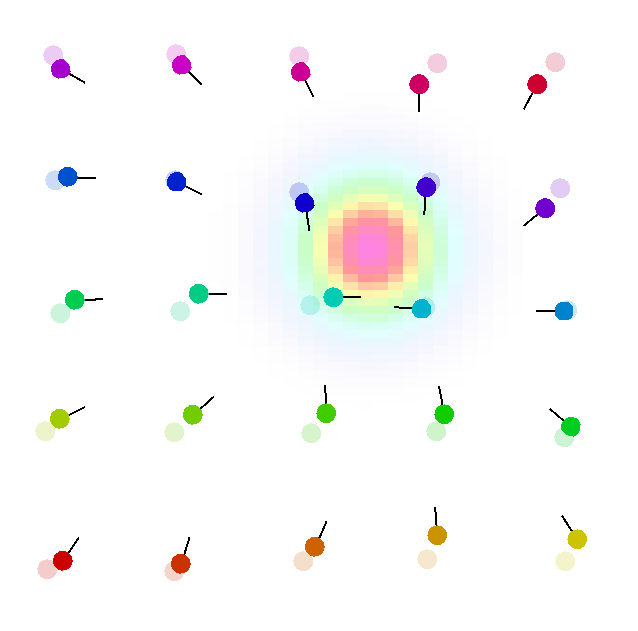
\includegraphics[width=\textwidth]{imgs/start.png}
		\caption{Start}
		\label{fig:initial}
	\end{subfigure}
	\begin{subfigure}[b]{0.32\linewidth}
		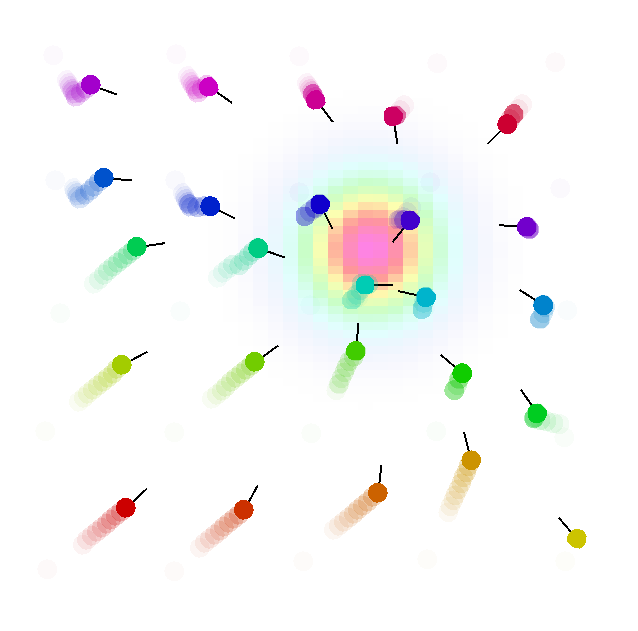
\includegraphics[width=\textwidth]{imgs/after.png}
		\caption{After 50 steps}
		\label{fig:after}
	\end{subfigure}
	\begin{subfigure}[b]{0.32\linewidth}
		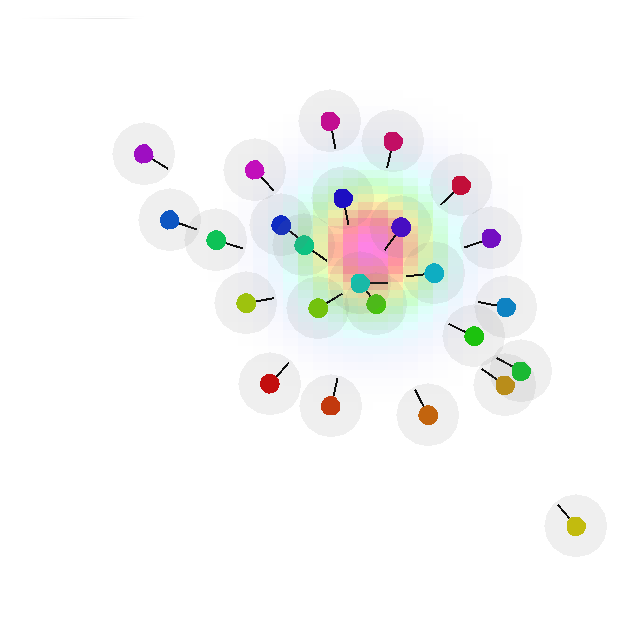
\includegraphics[width=\textwidth]{imgs/end.png}
		\caption{After 200 steps}
		\label{fig:end}
	\end{subfigure}
	\caption{Agents (coloured dots) are deployed in an area and have to coordinate to cover the phenomenon. The phenomenon can have varying areas of importance. Over time, the phenomenon will be covered sufficiently without any central controller.
%		
%		Qualitative test results of the proposed approach. 
%		The agents go towards the phenomenon and try to cover it without collapsing into a single point.
%		the grey area represents the area covered by the agents (last figure on the right).
		}
	\label{fig:simulations}
\end{figure}

%Specifically, 
% our approach utilises aggregate computing to disseminate information by manipulating a computational field, 
% which is a distributed data structure that maps devices to information. 
% This field functions as a dynamic environment in which information is continuously updated and diffused throughout the system. 
% By leveraging this layer, we can build collective distributed intelligence using \ac{GNN},
%  which uses the information in the field to determine the best action for a given task.
%\ga{first draft, need a refinement}
The remainder of this paper is structured as follows. 
 First, we introduce the relevant background and problem formulation in \Cref{sec:background}. 
 Afterwards, we introduce our approach in \Cref{sec:approach}. 
 \Cref{sec:eval} outlines the performed experiments and discusses the obtained results. 
 Finally, we will present our conclusions in \Cref{sec:conclusion}.

\section{Background and Motivation}
\label{sec:background}
%In this section, we aim to provide a concise overview of the system we intend to address, 
% starting with a high-level system model. 
%%
%We then proceed to discuss relevant research areas that inform our approach. 
%%
%Finally, we present a formalization of the problem and a discussion of the motivations behind our proposed work.
%\ga{Page budget: 1/2 page \\}
%\ga{Plan: discussion about the problem of coordination in multi-agent systems and the need for a scalable approach. In doing this, we will discuss some of the existing approaches (declarative, RL and )}
\subsection{Swarm systems}
This article studies intelligent \emph{collective behaviours} within the context of \emph{large-scale} distributed systems.
 Specifically, we focus on \emph{Cyber-Physical Swarms} or \emph{swarm-like systems} consisting of \emph{devices} governed by autonomous software \emph{agents} and equipped with \emph{sensors} and \emph{actuator} able to interact with the real world.
 Each of these agents can interact with its direct neighbours, either based on physical (e.g. communication range) or logical distance (e.g. 1-hop neighbourhood).
 
%
Each agent
 executes a \emph{local} control loop. 
 In each iteration of this loop, the agent can access the information available within its own \emph{context}. 
 This context is comprised of information acquired by the agent directly through its sensors and the information received from its neighbours. 
%
At the end of each control loop iteration, 
 the agent can send messages to its neighbourhood. 
 This message may contain raw sensor data or aggregated information over time or from other neighbours.
% about its current evaluation and update its internal state.
%
%This general model can be adapted to several different scenarios, such as a network of sensors, a network of robots (e.g., swarm robotics), or a network of mobile phones.
Examples of such large-scale systems can be a network of robots (e.g., swarm robotics), camera and IoT networks, or a network of mobile phones.
%
Our goal is to find a \emph{homogeneous} distributed controller $\pi$, namely the same controller for all agents of the system:
 starting from \emph{only} local configurations, it leads 
 the system to achieve a certain \emph{collective} requirement through \emph{cooperation}, 
 such as spatial area coverage, phenomena tracking, and robot aggregation~\cite{DBLP:journals/firai/SchranzUSE20}.
%
The homogeneity of the controller is a key requirement to ensure the \emph{scalability} of the approach, 
 as it allows us to avoid the need for a centralised controller that would be a bottleneck for the system,
 and it is the typical choice in swarm-like systems~\cite{brambilla2013swarm,yang2021many,pmlr-v80-yang18d,DBLP:conf/aaai/ZhengYCZZWY18}.
%
\subsection{Field-based Coordination}
%\ga{discussion about field used as a coordination mechanism in multi-agent systems. Introduction to AC}
The field-based coordination approaches utilise a concept of \emph{computational fields} 
 (or simply \emph{fields}), 
 which are \emph{distributed} data structures that associate each location with a computational value that evolves over time. 
%
\emph{Aggregate computing}~\cite{Beal2015Computer}, a modern field-coordination approach, is rooted in earlier work on \emph{artificial potential fields}~\cite{DBLP:conf/icra/Warren89} and \emph{co-fields}~\cite{DBLP:journals/pervasive/MameiZL04}. 
% 
This \emph{macro-programming}~\cite{DBLP:journals/corr/abs-2201-03473} paradigm can be realised to devise collective and self-organizing behaviour through a composition of functions operating on fields. 
%
The fields map a set of individual agents to computational values, 
 allowing them to associate what they sense, process, and actuate. 
%
Fields are computed locally but subject to a global viewpoint, 
 enabling emergent collective behaviour through the interplay of the \emph{system model} (i.e., structure and dynamics of the systems)
 and the \emph{programming model} (i.e., how collective behaviours are expressed).

On the one hand, the system model is structurally similar to \emph{swarm-like systems}, 
 as it is composed of a set of \emph{agents} 
 that interact with each other through a \emph{network} of \emph{neighbourhood relations}.
%
The dynamics of each agent follow a local control loop called \emph{round}
 that comprises the following steps:
\begin{enumerate}
  \item \emph{Sense}: the agent acquires information from the environment and collects the messages of its neighbourhood, building a \emph{context};
  \item \emph{Compute}: the agent executes a \emph{program} that computes an \emph{export}, that is a set of values to be sent to the neighbourhood;
  \item \emph{Act}: the agent sends the export to its neighbourhood and updates its internal state acting on the environment.
\end{enumerate}
The proactive and iterative execution of the round by each agent leads to the emergence of collective behaviour specified by the program.

On the other hand, the programming model is ruled by the \emph{field calculus}~\cite{DBLP:conf/esocc/ViroliDB13,DBLP:journals/corr/ViroliADPB16,DBLP:journals/tocl/AudritoVDPB19},  
 a core language that allows the expression of collective behaviours through the composition of \emph{functions} operating on fields.
%
Field calculus includes main operators for expressing \emph{spatio-temporal} computations that allow for 
\emph{i)} the progression of values over time, achieved by transforming a field computed in a previous round into a new field; 
\emph{ii)} the exchange of data with neighbouring fields (typically referred to as \lstinline|nbr|), where received data is accessed by adjacent fields; and 
\emph{iii)} the conditional division of computation into distinct domains of collective computation. 
%
%We avoid presenting here the full details of these operators since they are not essential to the contribution. 
For further elaboration on the actual field calculus, please refer to the work of~\cite{DBLP:journals/jlap/ViroliBDACP19}.

On these minimal operators, 
 it is then possible to build \emph{self-organizing} coordination blocks.
 One of the founding blocks is the \emph{gradient} essential for 
 \emph{information} flows~\cite{DBLP:conf/saso/WolfH07}.
%
This operator generates a numerical field that represents the minimum distance from a source zone. 
%
In other words, it maps a Boolean field (where ``true'' indicates the presence of a source agent and ``false'' indicates its absence) to a distance field that indicates the proximity to the nearest source. 
%
In ScaFi~\cite{casadei2022scafi} %(a scala implementation of aggregate computing)
 it is simply expressed as:
\begin{lstlisting}
def gradient(source: Boolean): Double
\end{lstlisting}
Along the gradient, it is possible to cast information within the system, accumulating value during the field expansion. 
This pattern is called \emph{gradient-cast} (or \emph{G}) and is a fundamental building block for the coordination of swarm-like systems.
It is expressed as: 
\begin{lstlisting}
def G[V](source: Boolean, value: V, acc: V => V): V
\end{lstlisting}
%\ga{more description here}
where \texttt{source} is a Boolean field indicating the presence of a source agent, 
 \texttt{value} is the value to be cast, and 
 \texttt{acc} is the accumulation function that is applied to the value during the cast.

%\lukas{Lukas to review this section again.}
\subsection{Graph Neural Networks}
%Over the years, several different neural networks have been proposed to solve specific tasks, ranging from 
%  simple \ac{MLP}~\cite{werbos1975beyond} to \ac{CNN}~\cite{oshea2015introduction}.
%  \lukas{more examples? }
%%
%Whereas \ac{CNN} is designed to be used with image and spatial-like data (e.g., audio), 
 \ac{GNN} is a novel neural network model used to process graph-structured data with deep learning approaches.
%
Let $G = (V, E)$ a graph  
where $E$ defines the neighbourhood relations for each participating node, 
and $V$ identifies the nodes present in the graph. %at that time.  \lukas{no time in the definition}
% 
Each node $v \in V$ is associated with an observation (or feature set) $f_v$.
For the sake of simplicity, 
 we thereafter describe $G_f$ as a graph that contains the feature set $f_v$ for each node $v \in V$.
 Note that, when we refer to $G_f$ and $G_o$ we are referring to the same graph $G$ but with different node features.
 Also, to access the feature set $f_v$ of a node $v \in V$ we use the notation $f_v$ or $G_f[v]$.
%\lukas{Over time this graph $G$ can change and therefore we define $G_t$ as the graph $G$ at a specific time $t$.} 
%
Given $f_v$, %a feature vector associated with each node $v \in V$, 
 the goal of a \ac{GNN} is to learn the node embedding $h_v$ for each node $v \in V$. 
 The node embedding $h_v$ describes the node in the network and summarises the geometric properties of the graph in this location, allowing for comparison of various nodes in the graph.
%
In modern \acp{GNN}, the node embedding $h_v$ is computed by aggregating information from the node's neighbours $\mathcal{N}_G(v)$,
 and then combining it with the node's current embedding $h_v$.
%
The graph is further partitioned into layers with the node $v$ at its bottom layer $0$. 
 With each traversal of an edge $e \in E$ from $v$, the number of layers increased
Formally, a \ac{GNN} can be defined by two phases:
\begin{equation}
a_{v}^{(k)}=\operatorname{AGGREGATE}^{(k)}\left(\left\{h_{u}^{(k-1)}: u \in \mathcal{N}_G(v)\right\}\right)   
\end{equation}

\begin{equation}
h_{v}^{(k)}=\operatorname{COMBINE}^{(k)}\left(h_{v}^{(k-1)}, a_{v}^{(k)}\right)
\end{equation}
where $h_{v}^{k}$ is the embedding of node $v$ within the $k$-th layer, 
 $\mathcal{N}_G(v)$ is the set of neighbours of node $v$ computed from $E$.
%
$h_v^0$ is the initial embedding of node $v$ and it is usually set to the node's feature vector $f_v$.
%
The differential part comes into play in the $\operatorname{COMBINE}$ function, 
 which is usually a differentiable function such as a neural network layer.
%
$\operatorname{AGGREGATE} $ instead is a function that aggregates the information from the neighbours of a node $v$
 and it could be a simple sum, max or sum of products. 
 More complex aggregation functions are available~\cite{pellegrini2020learning}.
%
Thereafter, we express the application of a \ac{GNN} to a graph $G_f$ as:
\begin{equation}
GNN(G_f) = \{h_v^{(k)}: v \in V, k \in \mathbb{N}\}
\end{equation} 
This formulation allows \acp{GNN} to effectively process and extract features from graph-structured data by iteratively aggregating and transforming information from the node's neighbours.
%\lukas{do we need definitions of $o_v$, $h_v^*$ over time $t$?}

\acp{GNN} are used in several application areas such as social network analysis, chemistry, and physics.
 In this paper, we use \acp{GNN} to learn a local behaviour for each agent in a multi-agent system (more details in Section~\ref{sec:approach}).
\subsection{Many-Agent Reinforcement Learning}
%\ga{plan: we could discuss briefly about standard approach (few agents), and mean-field approach (many agents). 
%This will lead to our approach, which is a combination of DQN (or any Deep RL approach) and GNN.}

 \Ac{RL} has gained a lot of interest recently, 
 thanks to its successful application in various scenarios, 
 ranging from video games (such as Alpha Go~\cite{Silver2016Go} and Atari~\cite{Atari2016DQN}) 
 to chatbots (like ChatGPT~\cite{ChatGPT2023}). 
% 
In \ac{RL}, an \emph{agent} (i.e., a smart entity capable of making decisions) 
 performs \emph{actions} in an \emph{environment} (i.e., everything outside the agent) according to a \emph{policy}, 
 to maximise long-term \emph{reward signal} (or minimise a \emph{regret}).

One interesting application of \ac{RL} is when there are multiple learning agents involved. 
 Such scenarios are referred to as multi-agent reinforcement learning (MARL)~\cite{zhang2019marl}. 
%
In particular, in this work, we consider homogenous \ac{MAARL}~\cite{yang2021many}, 
 where the set of agents is large ($N \gg 2$) and each agent is interchangeable and indistinguishable.
%
This research area is relevant in the context of large-scale systems 
 where collective intelligence emerges from local and repeated interaction of simple entities, like in swarm robotics.
%
In such many-agent scenarios, 
 the implementation of fully decentralized learning is often unfeasible due to the large number of learning agents, 
 which renders the system non-stationary and difficult to manage. 
%
Conversely, a centralized controller capable of coordinating 
 the entire system may not be a viable solution due to scalability concerns. 
 To address this challenge, a practical solution is the adoption of \ac{CTDE}.
%
The idea is to learn a policy at simulation time where there is a collective view of the system, 
 and then at runtime use the policy found with global information. 
This approach allows policies that are influenced by global information but only require local information to function at runtime. 
%
The typical approach in such cases is based on actor-critic systems~\cite{DBLP:conf/nips/LoweWTHAM17,wu2022more,song2022ctds,song2022centralized},
  where the \emph{actor} is the distributed policy (with only local information) and the critic is a neural network that takes the overall system state.
%
%In fact, the first works in this direction were discussed precisely swarm robotics, %\lukas{what does this mean `in the last field'?}
% exploring new models (e.g., swarMDP~\cite{DBLP:conf/atal/SosicKZK17}) and learning algorithms capable of extrapolating a policy representing the entire system.  \lukas{This sentence still needs rework.}
%Modern approaches, however, 
% have started to consider the use of 
% Recently, deep learning approaches have been considered 
% to synthesise robust controllers capable of generalizing to new tasks. 
%In this context, mean-field reinforcement learning~\cite{pmlr-v80-yang18d} is certainly noteworthy. 
Mean-field RL~\cite{pmlr-v80-yang18d} is one of such concrete applications of \ac{CTDE} 
 where the interactions among the population of agents are estimated by considering either the effect of a single agent and the average impact of the entire population or the influence of neighbouring agents.
%
Some known approaches using mean-field reinforcement learning include Q-mean, 
 which is an extension of Q-learning to mean-field settings~\cite{yang2018mean}, 
 and actor-critic mean-field~\cite{frikha2023actor}, which combines actor-critic algorithms with mean-field approximations. 
%
These approaches have shown promising results in various domains, such as multi-agent coordination 
 and decentralised control, and are actively being researched and developed for further applications.
\subsection{Problem formalisation}
Given the homogeneity, large system scale, and the \emph{locality} (i,e., each agent can only observe its neighbours), 
 the problem can be modelled through the SwarMDP model~\cite{DBLP:conf/atal/SosicKZK17} -- 
 an extension of the \ac{DecPOMDP}~\cite{Decpomdp2000} model for swarm-like systems.
% 
A SwarMDP is characterised by a \emph{swarming agent} ($\mathbb{A}$) and the dynamics of the environment ($\mathbb{E}$).
Specifically, $\mathbb{A}$ is a tuple ($\mathcal{S}, \mathcal{O}, \mathcal{A}, \mathcal{R}, \pi$) where:
\begin{itemize}
  \item $\mathcal{S, O, A}$ are the set of local states, observations (or features), and actions, respectively;
  \item $\mathcal{R}: \mathcal{S} \rightarrow \mathbb{R}$ is the reward function, which is influenced by the environment;
  \item $\pi: \mathcal{O} \rightarrow \mathcal{A}$ is the policy function, which maps the observations to the actions. It could be deterministic or stochastic.
\end{itemize}
Starting from this definition, the environment $\mathbb{E}$ is defined as a tuple ($\mathcal{P}, \mathbb{A}, \mathcal{T}, \xi$), where:
\begin{itemize}
  \item $\mathcal{P}$ is the total number of agents in the systems (the agent population), which is assumed to be fixed;
  \item $\mathbb{A}$ is the defined agent prototype that rules each agent $v \in P$;
  \item $\mathcal{T}: \mathcal{S}^P \times \mathcal{A}^P \times \mathcal{S}^P \rightarrow \mathbb{R}$ is the transition  global function, which is influenced by the actions of the agents and returns a collective reward -- this is typically not known by the swarming agents;
  \item $\xi: \mathcal{S^P} \rightarrow \mathcal{O^P}$ is the global observation model of the systems.
\end{itemize}
In swarMDP, the neighbourhood is not directly defined, but it is implicitly defined by the observation model $\xi$.
In our specific case, the agents can only interact with 1-hop neighbourhoods and are not directly influenced by other agent observations. We can therefore restrict the observation model as follows:
\begin{equation*}
\xi(v): \{s_j, j \in \mathcal{N}^v\} \rightarrow O
\qquad
\xi = \{\xi(v), v \in \mathcal{P}\}
\end{equation*}
where $\mathcal{N}^v$ is the set of neighbours of $v$.

This model can be used then to express the evolution of the system in time.
Specifically, starting from a global state $\mathcal{S}^P_t$, the next state $\mathcal{S}^P_{t+1}$ is defined as:
\begin{equation*}
\mathcal{A}^P_t = \pi(\xi(S^P_t))
\qquad
\mathcal{S}^P_{t+1} = \mathcal{T}(\mathcal{S}^P_t, \mathcal{A}^P_t)
\end{equation*}
Given a time $t$, the system can be also represented as a graph $G_t = (V_t, E_t)$, 
  where $E_t$ is built from $\mathcal{N}$.
  Each node is then decorated with the local observation perceived at the time $t$: $o^v_t \in O$. 
  Therefore, this graph can be used for being processed by a \ac{GNN} as done in~\cite{DBLP:conf/corl/TolstayaGPP0R19,tolstaya2020learning,DBLP:conf/icra/GosrichMLPYR022} if we set $f_v = o^v_t$.
\subsection{Motivation}
%The definition of distributed controllers for intelligent systems can be divided into two major approaches: 
% \emph{manual design}, where the application is conceived and described through a programming language, 
% and \emph{automatic design}~\cite{brambilla2013swarm}, which employs machine learning techniques to synthesise distributed controllers. 
%
%Our work lies between these two approaches, specifically in the areas of field-based coordination and \ac{MAARL} with the use of \acp{GNN}.
As mentioned above, our work falls between automatic and manual approaches, specifically in the areas of field-based coordination and \ac{MAARL} with the use of \acp{GNN}.
%
Compared to earlier works on field-based coordination, 
 our approach builds on the concept of co-fields~\cite{DBLP:journals/pervasive/MameiZL04}, 
 where agents exploit the field as a stigmergic medium to receive system-wide information and apply reasoning to this data.
%  
We present a subsequent approach where agent intelligence is synthesised through \ac{MAARL} and the use of \ac{GNN} to learn a local representation from the neighbourhood.
%
By learning a smart policy directly in the environment, the agent becomes capable of adapting its behaviour to new situations.

The use of \acp{GNN} as part of a distributed controller has been explored in previous literature~\cite{DBLP:conf/icra/GosrichMLPYR022,DBLP:conf/corl/TolstayaGPP0R19}, 
 where it was shown that they could be used to break down the evaluation of local and distributed systems. 
%
However, in these works, communication was left entirely to the neural network, 
 making the learning process potentially more complex and unstable. 
 In our approach, the \ac{GNN} is \emph{informed} by computational fields that collect the necessary information to compute a certain task, 
 limiting learning to only the specific task defined by a collective reward function.
 This will speed up the learning process and make it more stable.
\section{Field-informed Reinforcement Learning}
\label{sec:approach}
%\ga{Page budget: 2/3 pages \\}
%\ga{Plan: we should discuss the approach in detail, including the system model, and the learning dynamics. Particularly, I would like to highlight how each node in the graph is a local controller, but it could be seen as a global evolution, therefore we can use global information to inform the local controller.}
\begin{figure}
	\centering
  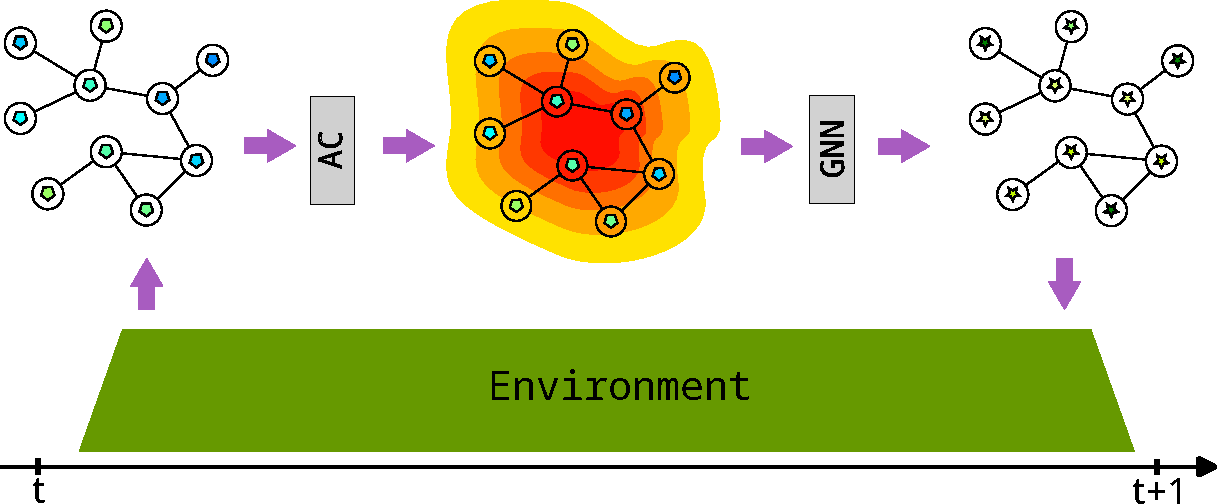
\includegraphics[width=.98\linewidth]{imgs/architecture.pdf}

  \caption{High-level description of \ac{FIRL} approach. 
  For each time step $t$, a graph is constructed from the environment, and it will associate each node with a local feature $o^v_t$ (hexagons in the picture). 
  Using this feature, an aggregate program computes spatio-temporal information that enhances the feature set of each agent producing $f_v$, depicted as colours in the middle graph. 
  Finally, utilizing the GNN, actions are computed for each agent in the system to be performed against the environment, enabling advancement in the simulations according to swarMDP rules.
  %\lukas{should we have numbers at each step in the figure (and then referring in the caption and text)?}
  %\lukas{also, i think we can have the AC and GNN box a bit smaller but increase the size of the networks slightly - and put it on column width ot save space}
}  \label{fig:architecture}
\end{figure}
In this section, we discuss the components involved in our proposed solution (i.e., architecture) and how these components interact with each other to bring the system to perform the collective behaviour (i.e., dynamics). Finally, we will detail the learning algorithm designed and used to synthesise the policy.
\subsection{Architecture and System dynamics}
%\ga{Plan: 
%  discussion about the typical AC evaluation model, specifying how GNN (with 1-hop information diffusion)
%  can be easily integrated with this distributed model
%}
The proposed solution, summarised in \Cref{fig:architecture}, consists mainly of two parts, 
\emph{i)} the aggregate program used to create part of the observation and 
\emph{ii)} the policy $\pi_{gnn}$ learned through \ac{GNN}-based approach. 
%
Let $\Gamma$ be the aggregate program that takes a graph $G_t$ decorated by $o^v_t$, 
 representing the participating agents and their neighbourhood relations at time $t$, as input. 
% \lukas{$G_t$ is not defined. also, not sure what `runs against' means - take $G_t$ as input?}
%\ga{In the problem formalization, I defined $G_t$, but it may be more appropriate to define it directly in the GNN, as suggested. I made this choice since GNNs typically only receive a graph as input, without regard for time, I included the definition of $G_t$ in the problem formalization as it pertains to the dynamics of the overall system. Specifically, when discussing the system's dynamics at a given time t, it's necessary to define the corresponding graph. I hope this clarifies my reasoning. Let me know!}
%
The evaluation of $\Gamma$ produces a field value $\theta^v_t$ for each node $v$ in $G_t$. 
From this field, we construct the feature vector $f_v$ for each node $v$ in $G_t$ as follows:
 $f_v = (\theta^v_t, o^v_t)$.
%  \lukas{we used $o_v$ to describe the observation of node $v$ in section II.C - so this would not include field information, right?}
% \lukas{we have not introduced $G'_t$ yet}
 %where $\omega$ are other local information gather from sensors (like temperature, distances from neighbourhood, etc.). 
%
The policy $\pi_{gnn}$ is then evaluated for each agent using $f_v$ as input, 
 producing an action $a^v_t$ that will then modify the global state of the system.
 %\ga{todo: put pseudo code to express this dynamics}
%
While the graph, containing the aggregate information, 
 might appear as global knowledge, 
 this is not the case as the information is never aggregated globally. 
The individual agents only combine information from their local neighbourhood.
%
In fact, the program $\Gamma$ is proactively executed at every agent, 
and the \ac{GNN} can be locally evaluated using only neighbourhood information. 
%
We want to emphasise that, in this case, the \acp{GNN} must be 1-hop; 
otherwise, they could not have a local interpretation for each agent, according to our system model.
\subsection{Learning algorithm}
%\ga{
%  Plan: discuss the chosen approach, that is Centralised Training and Distributed Execution.
%  Particularly, we use DQN in which the neural network is a GNN. So, the dataset consists in a set of graphs,
%  where each graph is a snapshot of the system. 
%  The target is the Q-value of the action taken in the current state.
%  Explain how this can be then used for distributed controllers.
%}
Since we consider swarm-like systems, which are an example of many-agent systems, 
 the proposed approach follows a \ac{CTDE} learning pattern,
 but differently from mean-field approaches and actor-critic solutions,
 we use a \emph{value-based} approach combined with a \ac{GNN} as a function approximator.
%In swarm-like systems, 
% the typical approach for learning follows a strategy known as \ac{CTDE}. \ga{perhaps it should be introduced in many RL} 
%The idea is to learn a policy at simulation time where there is a collective view of the system, 
% and then at runtime use the policy found with global information. 
%This approach allows policies that are influenced by global information but only require local information to function at runtime. 
%
%The typical approach in such cases is based on actor-critic systems~\cite{DBLP:conf/nips/LoweWTHAM17,wu2022more,song2022ctds,song2022centralized},
%  where the \emph{actor} is the distributed policy (with only local information) and the critic is a neural network that takes the overall system state.
%
Specifically, we leveraged the property of \ac{GNN}s to have a dual interpretation, 
i.e., to function globally over the entire graph and locally only over the neighbourhood. 
Importantly, each agent only has local information from itself and its neighbourhood to utilise in the \ac{GNN}.
% \lukas{Global information is not available to the agent, right? The agent only provide locally aggregated information (resulting from the AC part)?}
%
As value-based algorithm we relied on \ac{DQN}~\cite{mnih2015playing} %\ga{to introduce in many rl??} 
with two major modifications (see \Cref{alg:dqn}): 
\begin{enumerate}
  \item experience replay stores experiences in the form of \emph{graphs} decorated with features (e.g., observations, actions, rewards, etc.),
  \item the neural network used to compute the Q function is based on a \ac{GNN} with an \ac{MLP} downstream.
\end{enumerate}
The first point is a natural extension because we work on graphs rather than simple values.
This also influences how we create a batch of experiences to train the network.
 In fact, we sample a batch of graphs from the replay buffer,
 and then we merge them into a single graph,
 which is then used to train the network.
 This process is called \emph{graph mini-batching}~\cite{DBLP:journals/corr/abs-1903-02428,wang2019deep}
 and its main purpose is to pass an entire batch of graphs to the same \ac{GNN} for improved performance.
%
For the second point,
 the use of \acp{GNN} allows us to define policies on a variable neighbourhood, which is essential in such systems as this can change due to the applied neighbourhood policy.
 It is known that \acp{GNN} have a certain ability to generalise to new structures and scale with different agents~\cite{DBLP:journals/aiopen/ZhouCHZYLWLS20,DBLP:conf/nips/KnyazevTA19}. 
% 
Additionally, 
 using the overall graph compared to local experiences makes learning more stable as it reduces the non-stationarity of the environment perceived by each node.
% 
This is because, even though the actions are produced using only local and neighbourhood information, 
 during the learning phase, we have access to the internal graph, 
 which will influence the policy through non-local information 
 during the backpropagation.
%
\begin{algorithm}
  \KwIn{Environment $\mathbb{E}$, graph replay buffer $\mathcal{D}$, target network $\theta^{-}$, current network $\theta$, exploration strategy $\epsilon$}
  \KwOut{Trained DQN model $\theta$}

  Initialise $\mathcal{D}$ with random initial transitions;

  Initialise $\theta$ with random weights;

  Set $\theta^{-} \leftarrow \theta$;

  \While{not done}{
  Observe current graph observations $G_o$;

  \uIf{random $< \epsilon$}{
    select a random action $a$;
  }
  \Else{
    $G_q = Q(G_o, \theta)$;
    $a = \{ v \in G_q | a_v \in argmax_{a_v} G_q[v](a_v) \}$;

  }

  Execute the collective action $G_a$ in the environment $\mathbb{E}$ and observe a graph-level reward $G_r$ and the next observation $G_o'$;

  Store transition $(G_o,G_a,G_r, G_o')$ in $\mathcal{D}$;

  Sample a batch of graph transitions $(G^i_o,G^i_a,G^i_r,G'^i_o)$ 
   from $\mathcal{D}$ and merge them in $(G^b_o,G^b_a,G^b_r,G'^b_o)$; 

  Compute the target Q-value for each node $v$ in the graph $G^b$: 
  $y_v = G^b_r[v] + \gamma * \max{a'} Q(G'^b_o[v],G^b_a[a'];\theta^{-})$;
  
  Compute the current expected value for each node $v$ in the graph $G^b$:
  $y_v^* = Q(G^b_o[v],G^b_a[v];\theta)$;

  Update the current network weights using gradient descent: $\theta \leftarrow \theta - \alpha \nabla{\theta} \frac{1}{|G^b|} (y - y^*)^2$;

  Every $C$ steps, update the target network weights: $\theta^{-} \leftarrow \theta$
  ;
  }
  \caption{Deep Q-Network (DQN) with GNN and Graph Replay Buffer executed by each agent}
  \label{alg:dqn}
  \end{algorithm}
 
    
\section{Evaluation}
\label{sec:eval}
\begin{figure}
  \centering
  \begin{subfigure}[b]{0.32\linewidth}
      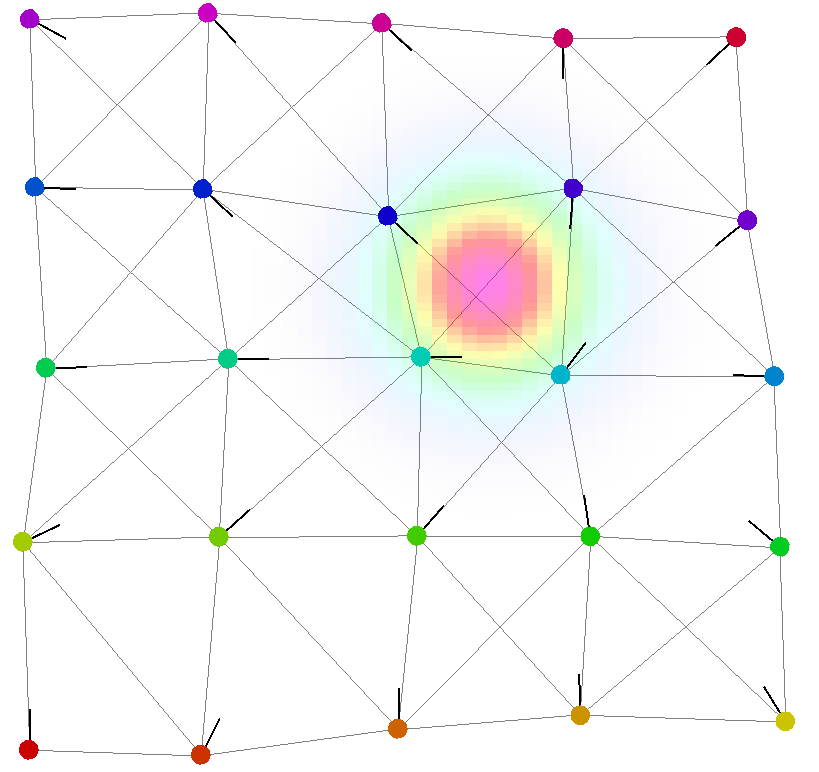
\includegraphics[width=\textwidth]{imgs/example.png}
      \caption{}
      \label{fig:static}
  \end{subfigure}
  \begin{subfigure}[b]{0.32\linewidth}
      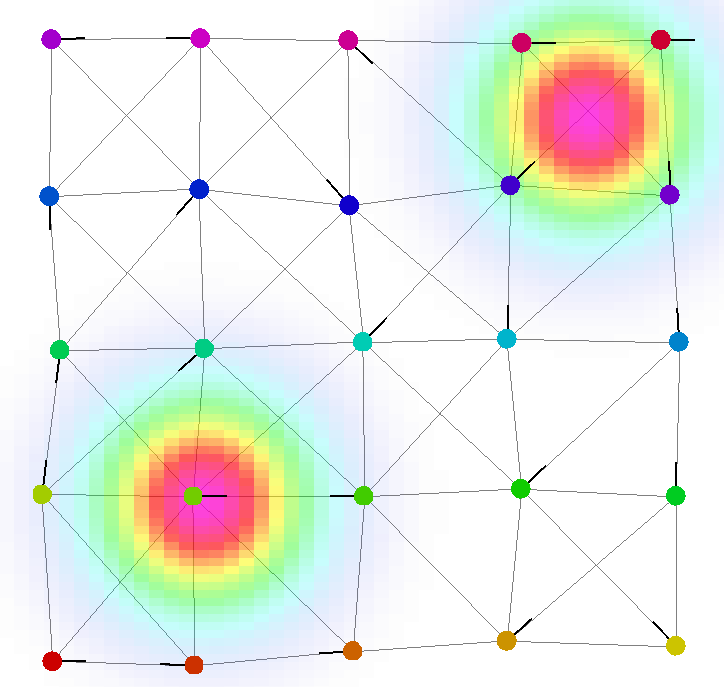
\includegraphics[width=\textwidth]{imgs/two-zones.png}
      \caption{}
      \label{fig:two}
  \end{subfigure}
  \begin{subfigure}[b]{0.32\linewidth}
      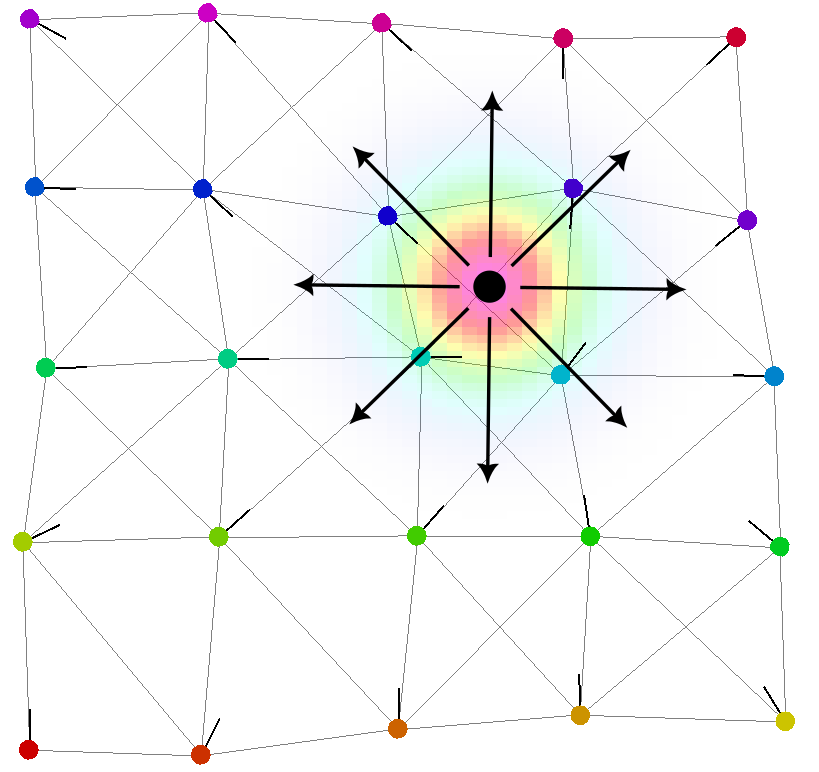
\includegraphics[width=\textwidth]{imgs/example-moving.png}
      \caption{}
      \label{fig:moving}
  \end{subfigure}

  %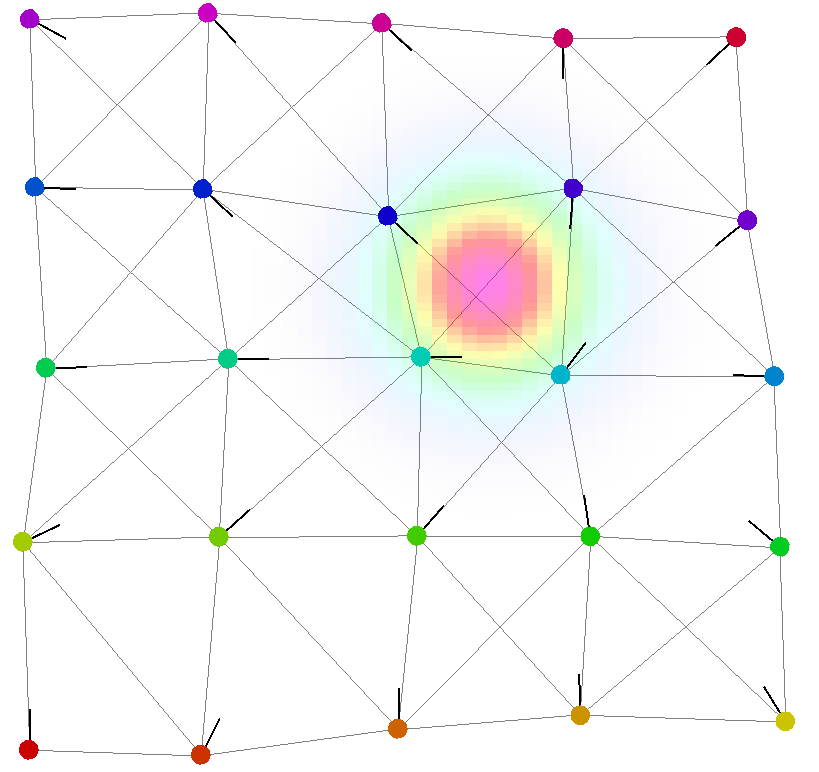
\includegraphics[width=0.3\textwidth]{imgs/example.png}
 
  \caption{Simulations of the case study scenario in Alchemist. 
  The dots represent the agent, 
  the circle area on represents the phenomenon to be monitored.
  \Cref{fig:static} represents the scenario used during training. 
  The others are used in the test phase to evaluate the policy found. }
  \label{fig:scenarios}
\end{figure}
%\ga{Page budget: 2 pages \\}
%\ga{Plan: we should discuss the robot aggregation scenario, specifying the state space, the action space, and the reward function.
%I dunno if it makes sense to discuss the variants (i.e., fixed area, two areas and moving area). We will see.}
To test the effectiveness of the proposed approach, 
 we decided to experiment with a case study related to swarm robotics, 
 specifically the tracking and coverage of a spatio-temporal phenomenon, cf. tracking a wildfire 
 or monitoring the water levels in a canal with multiple autonomous agents embodied in embedded devices (e.g., drones or IoT devices). The individual agents do not have any knowledge of the initial phenomenon itself (i.e., shape, size, location, velocity,...).
 %
Initially, 
  we perform the training phase using a stationary phenomenon before expanding towards a moving phenomenon in the test phase. 
  %Additionally, the phenomenon can change its shape during runtime. 
  Finally, the phenomenon may have varying areas of interest, defined by an underlying distribution function. This underlying distribution is utilised in the feature set of each agent's observation and guides the agents to rally over the phenomenon. While we only use Guassian distributions but we can use any other distribution and shape. 
As a simulation environment, we use Alchemist~\cite{alchemist}, 
 a simulator for multi-agent systems that allows us to simulate the swarm behaviour of the agents 
 and the phenomenon of interest.
For the \ac{GNN}, we use the implementation provided by PyTorch Geometric~\cite{Fey/Lenssen/2019}, 
 which is a library for deep learning on graphs built on top of PyTorch~\cite{torch}.
Finally, we use ScaFi~\cite{casadei2022scafi} as the aggregate programming language to support our field-informed approach.
The evaluation is performed in two stages, first the neural networks are trained in an explicit training phase before being extensively evaluated in the testing stage.
\footnote{The simulations are publicly available at \url{https://github.com/AggregateComputing/experiment-2023-acsos-field-informed-rl}.}
\subsection{Scenario}
\Cref{fig:scenarios} presents the three different types of scenarios utilised within the evaluation. The first type of experiments considers a single phenomenon at a static location (i.e., \emph{Zone Fixed}), the second type of experiment considers two phenomena in two independent but static locations (i.e., \emph{Two Zones}), and the third type of experiment considers a moving phenomenon (i.e., \emph{Moving}). All phenomena are modelled as a Gaussian distribution. Importantly, only the left scenario illustrated in Figure~\ref{fig:static} was used for training the neural networks. 
Furthermore, all three types of scenarios contain a set of $\mathcal{P} = 25$ agents placed in a 2D grid large 1000x1000 meters. % and a single, stationary phenomenon with a  
Each agent can perceive the presence
 of the phenomenon of interest through an installed sensor $\zeta_v$ with $v \in \mathbb{V}$. 
 (e.g., camera, temperature sensor, etc.) if it is within range.
%
Additionally, each agent has a coverage range $\omega$ (fixed to 75 meters) 
 that describes the area it can monitor. 
 Each agent can only communicate directly with its own neighbourhood $\mathcal{N}$, 
 which in this case depends on a $\mathbb{O}$ range fixed to 300 meters. %\lukas{$\mathbb{O}$  not defined.}
Through this communication channel, agents can exchange information. 
%From the neighbourhood, each agent can also perceive the direction of the other agents.
%
Each agent moves following a certain action composed of two components (r, i) 
 which respectively describe the angle and intensity of the movement (i.e., the velocity vector).
Since we used a value-based approach, 
 the action space $\mathcal{A}$ is discrete and composed of 18 possible angles and 3 possible intensities.
In particular, the angles are quantized to 20 degrees, and for the velocities, we have selected [0, 5, 10] m/s.
%\lukas{is this training the \ac{GNN}? }, 
%

For the aggregated information, each agent will produce a computation field with which they will try to approximate the direction of the phenomenon of interest. 
%
%
%The specific program in question is a simple application of block G, where the source is the maximum value of the neighbourhood. 
The program $\Gamma$ in question is a simple application of block G, where the source is the maximum value of the neighbourhood. 
This can be expressed in Scafi as follows:
\begin{lstlisting}[mathescape=true]
val source = maxHood(nbr(sense($\zeta$))) == sense($\zeta$)
G(source, Point3D.Zero, _ + nbrVector())
\end{lstlisting}
where \texttt{maxHood} is a function that returns the maximum value of the neighbourhood, 
 \texttt{nbr} is a function that returns the value of the neighbourhood, 
\texttt{sense} is a function that returns the value of the sensor, and
\texttt{nbrRange} is a function that returns an approximate direction for each agent in the neighbourhood.
%
This value will then be fed into the $\pi_{GNN}$ to compute the action to be performed.
 %\lukas{not sure if this paragraph should be its own subsection. or at least it needs  different title.}

 
 %\lukas{drone, robot, agent, node...}
\subsection{Goal}
 The objective of this scenario is threefold:
\begin{enumerate}
\item Maximise the number of agents within the phenomena
\item Minimise the number of agents without a neighbourhood
\item Maximise the coverage of the system
\end{enumerate}
 
As we are modelling a reinforcement learning system, 
 these three components must be encoded in a reward function 
 that provides an estimate of the current action taken by a given agent.
 
% Regarding the first point, the reward function is simple and is defined as:
Formally, we define the reward of an agent being within the phenomenon as
 \begin{equation*}
 R^a_{v} = \begin{cases}
  1 & \text{if } \zeta_v > 0 \\
  0 & \text{otherwise.} 
 \end{cases}
 \end{equation*}
Namely, an agent is considered within the phenomena as soon as the drone can sense the phenomenon.
%
This will lead the system to prefer a configuration in which every agent is present within the phenomenon.
%
The second element in the objective function ensures cohesion among the agents. 
 This is important because if the system breaks into many scattered agents, 
 the observability of the phenomenon is reduced, 
 limiting the ability of the agents to move appropriately in the environment.
% they are not able to move in the environment due to the reduced observability of the system. 
 In this case, the reward is defined as:
 \begin{equation*}
 R^{\mathcal{N}}_{v} = \begin{cases}
  1 & \text{if } \mathcal{N} > 0 \\
  0 & \text{otherwise} 
 \end{cases}
 \end{equation*}
 
Finally, to maximise the coverage, 
  we define a reward function that favours the maximum distance between the agents
  equal to the coverage range $\omega$. This will minimise multiple agents covering a common area.
%
This means that the average distance will tend towards the one expressed by the viewing range of each agent:
% 
\begin{equation*}
R^{C}_{v} = 1 - \frac{d_{min}}{\omega}
\end{equation*}
where $d_{min}$ describes and minimum distance of the agent to its neighbourhood. 
%
%\lukas{should this be $1-R^C_v$? or do we want to favour the highest average distance?}
The final reward function $R_{v}$ for an agent $v$ is defined as:
\begin{equation*}
R_{v} = (\frac{R^a_{v} + R^{\mathcal{N}}_{v} + R^{C}_{v}}{3}) - 1
\end{equation*}
Specifically, we decided to express the signal as a \emph{regret}
  as it is a more general measure of the quality of the action taken by the agent.
%
\subsection{Training Phase}
Before we can evaluate our approach, the underlying neural networks have to be fine-tuned in a dedicated training phase.
The training process for each neural network was divided into 100 episodes, each consisting of 200 steps, resulting in a total of 20,000 experiences.
%
For each episode, 
 the 25 agents are semi-randomly positioned on a grid (i.e., in a lattice layout with a random variation in their position) without knowing the correct position of the phenomenon, 
 but that is fixed in the top right corner. The position of the phenomenon with an example of positioned agents can be seen in Figure~\ref{fig:static}. 
% \lukas{so for all 20,000 experiences, the phenomena is exactly as shown in fig 2a during training? --> WE ONLY USE THE SINGLE PHENOMA IN A SINGLE FIXED LOCATION BUT WITH VARYING POSITIONS OF AGENTS!!}
 The feature set used by the \ac{GNN} created for each agent consists of the vector computed by the aggregated program and the value of the local sensor $\zeta$.
%
In this case, we chose to use an exponential epsilon decay, defined as:
\begin{equation*}
\epsilon = \epsilon_{min} + (\epsilon_{max} - \epsilon_{min}) \cdot e^{-\lambda \cdot e}
\end{equation*}
where e is the current episode number. 
This leads to a high number of random actions at the beginning and gradually shifts towards exploitation in the later episodes. 
%
In our training process, 
 we set $\epsilon_{min} = 0.02$, $\epsilon_{max} = 0.99$, and $\lambda = 0.1$.
$\gamma$ was set to 0.99, 
 as we want to give more value to future returns, 
 aiming to achieve good coverage by continuously tracking the phenomenon. 
The neural network structure used consists of a layer of SuperGAT~\cite{DBLP:journals/corr/abs-2204-04879} -- A \ac{GNN} based on attention mechanisms -- and a layer of MLP. 
The hidden size was set to 256.
%
As the reward function is defined as a regret, 
 we decided to use the Huber loss function with $\delta = 1$, %~\cite{??}, 
 %which is a combination of the $L_1$ and $L_2$ loss functions.
%
%The loss function is defined as:
%\begin{equation*}
%L_\delta = \begin{cases}
%  \frac{1}{2} (y - \hat{y})^2 & \text{if } |y - \hat{y}| < \delta \\
%  \delta \cdot (|y - \hat{y}| - \frac{1}{2} \delta) & \text{otherwise,} 
% \end{cases}
%\end{equation*}
%where $\delta$ is a hyperparameter that determines the threshold between the two loss functions (fixed to 1 in our experiemnt) and $y$ and $\hat{y}$ are the target and predicted values, respectively.
This function is used to penalise the agent if the action taken is too far from the optimal action. 
%\lukas{what is the value of $\delta$ in the training?}
%\lukas{also: $\delta$ is used as a function and as a value?}
%
We use the RMSprop optimiser with a learning rate of 0.0001.
%
Finally, we use a replay buffer of size 1000 to store the graph experiences and a batch size of 32.
\subsection{Test phase}
For the evaluation, 
 we explore the previously discussed three different types of experiments.
%%
%The first type considers only a single, stationary phenomenon like the one used in the training phase. 
%%
%The second type considers multiple phenomena, requiring the agents to make a decision about which phenomena to cover. 
%%
%Finally, the third type considers a single moving phenomenon which the agents have to follow throughout the simulation. 
%%
%In all three types of scenarios, the shape and underlying distribution are initially unknown to the agents but remain constant for the entire duration of the simulation. 
%
We generated 64 random scenarios for each type of experiment. 
 Additionally, the placement of the agents was randomised as it has been done during training.
For the first type, consider a single static phenomenon randomly placed in the environment. 
This is in contrast to the training where the phenomena were always placed in the same location.  
For the second type, we placed two distinct phenomena within the area. 
Their location is kept constant in all 64 experiments. 
As the training only contained a single phenomenon, 
this setup represents a challenge for the agents.
Finally, the third type contained moving phenomena. 
In each scenario, the starting position as well as the direction of movement is randomly sampled from a uniform distribution. 
The movement is in a straight line with a constant speed of 5m/s within an unbounded environment. 
%to ensure the agents can keep up with the phenomenon. 
%\lukas{64 experiments per mode with random initial positions of the phenomena. Moving: starting at random position and move in a straight line moving with 5m/s in an unbounded environment.}
%
Examples of all three types of experiments are shown in~\Cref{fig:scenarios}. %\lukas{can we create a figure with at least 3 sample scenarios (1 stationary, 2 split, 1 moving (with a line indicating its trajectory))?} 

%\lukas{I would move this up into IV.A --> emphasise that we only used a single static phenomena in the training therefore this section is improtant!}

\subsection{Baselines}
We compare our \ac{FIRL} approach against baseline approaches where the \ac{DQN} utilises a \ac{MLP} as well as an approach only relying on \acp{GNN}, without additional field information. 
%
In all approaches, the underlying neural network (i.e., the \ac{MLP} and the \ac{GNN}) are trained %with the same parameters of the proposed approach 
with a single, stationary phenomenon.
%

The \ac{MLP} uses the same feature set as the \ac{GNN} but applies it in the \ac{DQN} but 
%in the proposed approach, but differently, it uses a standard DQN approach 
without leveraging the graph structure. Moreover, we increase the batch size to 512 and the replay buffer to 10000 since we record 25 agents' experiences for each step instead of one graph experience.
%\lukas{to make sure: in all three cases we use DQN but with (i) MLP, (ii) standard GNN, (iii) our approach - a field-informed GNN, right?}
%
%The \ac{GNN} instead of using the field information, use directly the position of nodes and the local sensor value as input features.
The \ac{GNN} alone, without using the field information, apply the position of agents and the local sensor value directly as input features within the \ac{DQN}.
%
These baselines are used to verify the effectiveness of the components used in the field-informed \ac{RL}. 
%
Indeed the \ac{MLP} baseline is used to verify the effectiveness of the \ac{GNN} in the proposed approach, while the \ac{GNN} baseline is used to verify the effectiveness of the field information in the proposed approach.
\subsection{Metrics}
We evaluate the performance of the different approaches by measuring the coverage of the phenomenon over time.
%
The coverage is defined as the percentage of the phenomenon covered by the agents.
%
Specifically, we can measure the coverage as the intersection over the union of the phenomenon and the agents' view range.
%
Formally, first, we define the overall coverage for a certain time step as:
\begin{equation*}
\Omega = \bigcup_{v \in V} \omega_v
\quad 
C = \frac{|\Omega \cap \mathcal{P}|}{|\mathcal{P}|}
\end{equation*}
where $\mathcal{P}$ is the area of the phenomenon and $\Omega$ is the area covered by the agents.
%This is computed for each step of the simulation. 
In the training phases, 
 we measure the average coverage in each episode, and the total reward obtained by the agents at each episode of the simulation. 
%
We also measure the number of agents that are within the phenomenon at each step of the simulation.
This will be a measure of how well the agents are tracking the phenomenon.
%\ga{todo improve the description of the coverage}

\subsection{Discussion and Results}
The results of the training process are summarized in \Cref{fig:training}. 
%
Specifically, we observe that the proposed version achieves higher coverage and total reward compared to other approaches. 
%
Interestingly, despite the global information available in \acp{GNN} without fields, they fail to converge to a good result like the one obtained with the field. 
%
This outcome was expected, as the computed field helps agents encode the necessary information to navigate towards the phenomenon.
%
Furthermore, we note that \ac{GNN} combined with \ac{DQN} and graph replay buffer outperforms the simple \ac{MLP} informed field computation. 
%
This is because relying solely on \ac{MLP} and basic deep learning leads to non-stationary and unstable learning, 
 as evident from the wider confidence interval of the reward over training time.

Focusing now on the results of the test phase, highlighted in  \Cref{fig:test},
 we observe that the field-informed version achieves higher coverage than the other approaches in all scenarios since it shows the ability of our solution to generalize to situations. 
% 
We observe that the field-informed version successfully moves the agents closer to the target phenomenon, 
 distributing them evenly without collapsing into a single central point. 
 \Cref{fig:test} quantitatively presents the results across various previously described scenarios.

For all experiments, both \ac{GNN} versions demonstrate the capability to transfer the learned experience to the test phase whereas the MLP version fails to generalize. 
%
It is worth noting that, in the \emph{Zone Fixed} experiment, % (left graph in \Cref{fig:test}), 
 once the desired configuration is achieved in the static case, 
 the agents cease to move, maintaining the found configuration.
%
Interesting observations arise when we use scenarios different from the training phase. 
% Starting from a division into two zones, 
In the \emph{Two Zones} experiment,
 we notice that our approach using field-information finds a better configuration than the simple GNN counterpart. 
%
It exhibits both higher overall coverage and manages to divide the system into two equally covered parts. 
%
Indeed, observing the \Cref{fig:resCoverage}, we notice that the informed version maintains a balanced coverage between the two zones, 
 with a difference of less than 5\% between the two parts, maintaining a fair division of the phenomena.
%
In contrast, the uninformed version also maintains a fair division but with significantly different coverage between the two parts, 
 indicating a wrong placement among the agents in one of the zones.
%
This is a consequence of the uninformed version's inability to encode the necessary information to divide the agents into two zones, therefore it is not able to generalise.
%
Finally, the \emph{Moving} experiment emphasizes how the informed version generates a more robust policy for new scenarios. 
 Indeed, we observe that our approach using \ac{FIRL} maintains higher coverage and a greater number of agents on the target phenomenon compared to the other two solutions.
%
The uninformed GNN version, however, 
 fails again to generalize its movement behaviour, as evidenced by the simulations where the agents, once reaching the target zone, stop moving due to tracking issues.

In conclusion, the results demonstrate how the proposed idea can generate more robust controllers. 
 By guiding information flow in \acp{GNN}, 
 we improve learning efficiency and alleviate the challenge of encoding relevant information. 
%
Nevertheless, we acknowledge the crucial role of \acp{GNN}. 
 Our modified version of DQN, combined with \acp{GNN}, 
 enables the discovery of robust behaviours in a few episodes, 
 which is challenging to capture with \acp{MLP} combined with \ac{DQN}, even if we use field information.
% \lukas{add short discussion on 'new' figure 6}
\begin{figure}
  \centering
  \hfill
  \begin{subfigure}[b]{0.87 \linewidth}
    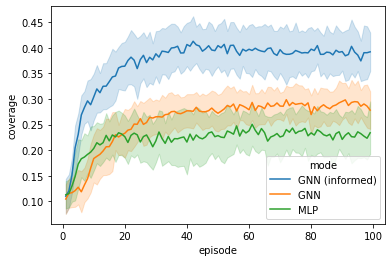
\includegraphics[width=\linewidth]{imgs/coverage-in-time}
    \caption{Average coverage for each episode in training }
    \label{fig:coverage}
  \end{subfigure}\\
  \hfill
  \begin{subfigure}[b]{0.9\linewidth}
    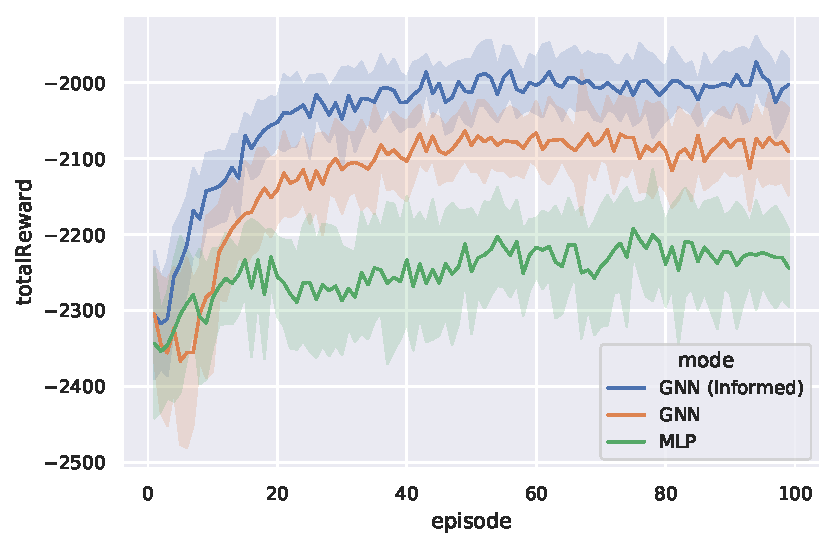
\includegraphics[width=\linewidth]{imgs/reward-in-time}
    \caption{Reward during training}
    \label{fig:reward}
  \end{subfigure}
  \caption{Training results of field-informed \ac{RL}. 
  Our solution is able to cover the phenomenon better than the baselines and it reaches a higher reward. 
  }
  \label{fig:training}
\end{figure}


%% Create a subfigure of coverage-test, inside-test, inside-two-test and coverage-two-test

\begin{figure*}
  \centering
  \begin{subfigure}[b]{0.9\linewidth}
    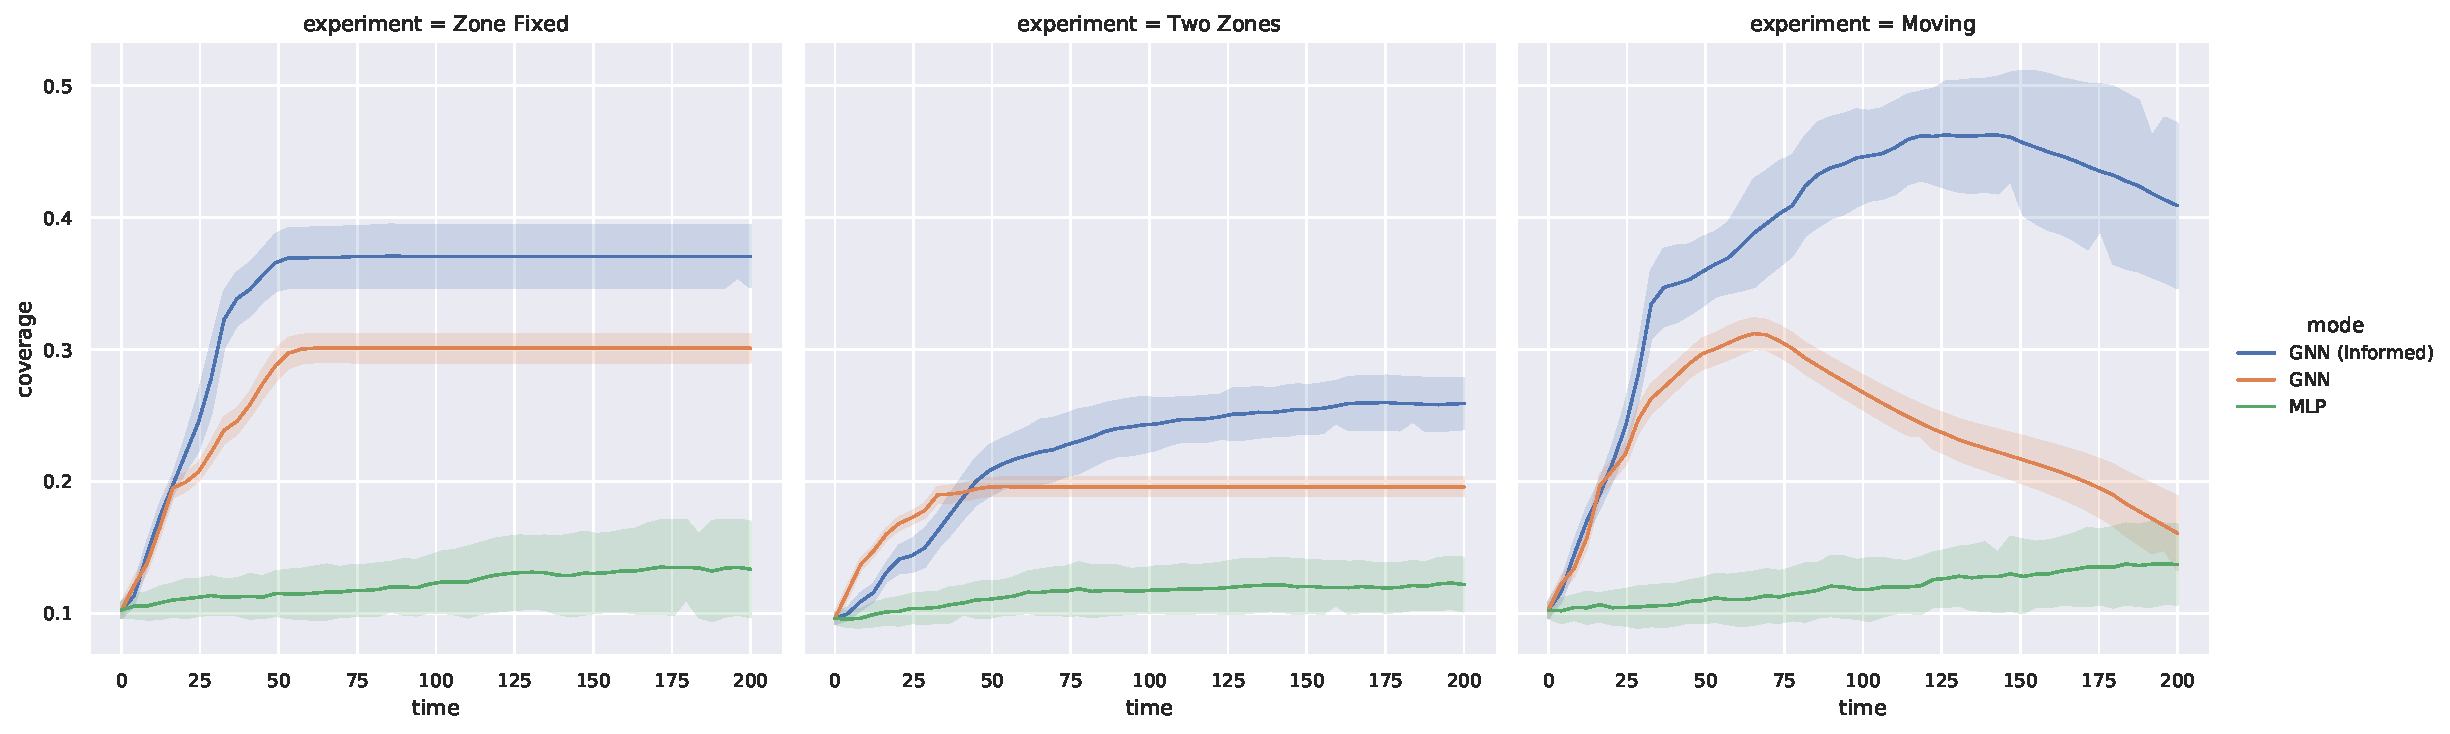
\includegraphics[width=\linewidth]{imgs/coverage-test.pdf}
    \caption{Ratio of coverage of the phenomena in the three types of experiments. Our \ac{FIRL} approach can outperform other approaches lacking field information.}
    \label{fig:coverage-test}
  \end{subfigure}
  \begin{subfigure}[b]{0.9\linewidth}
    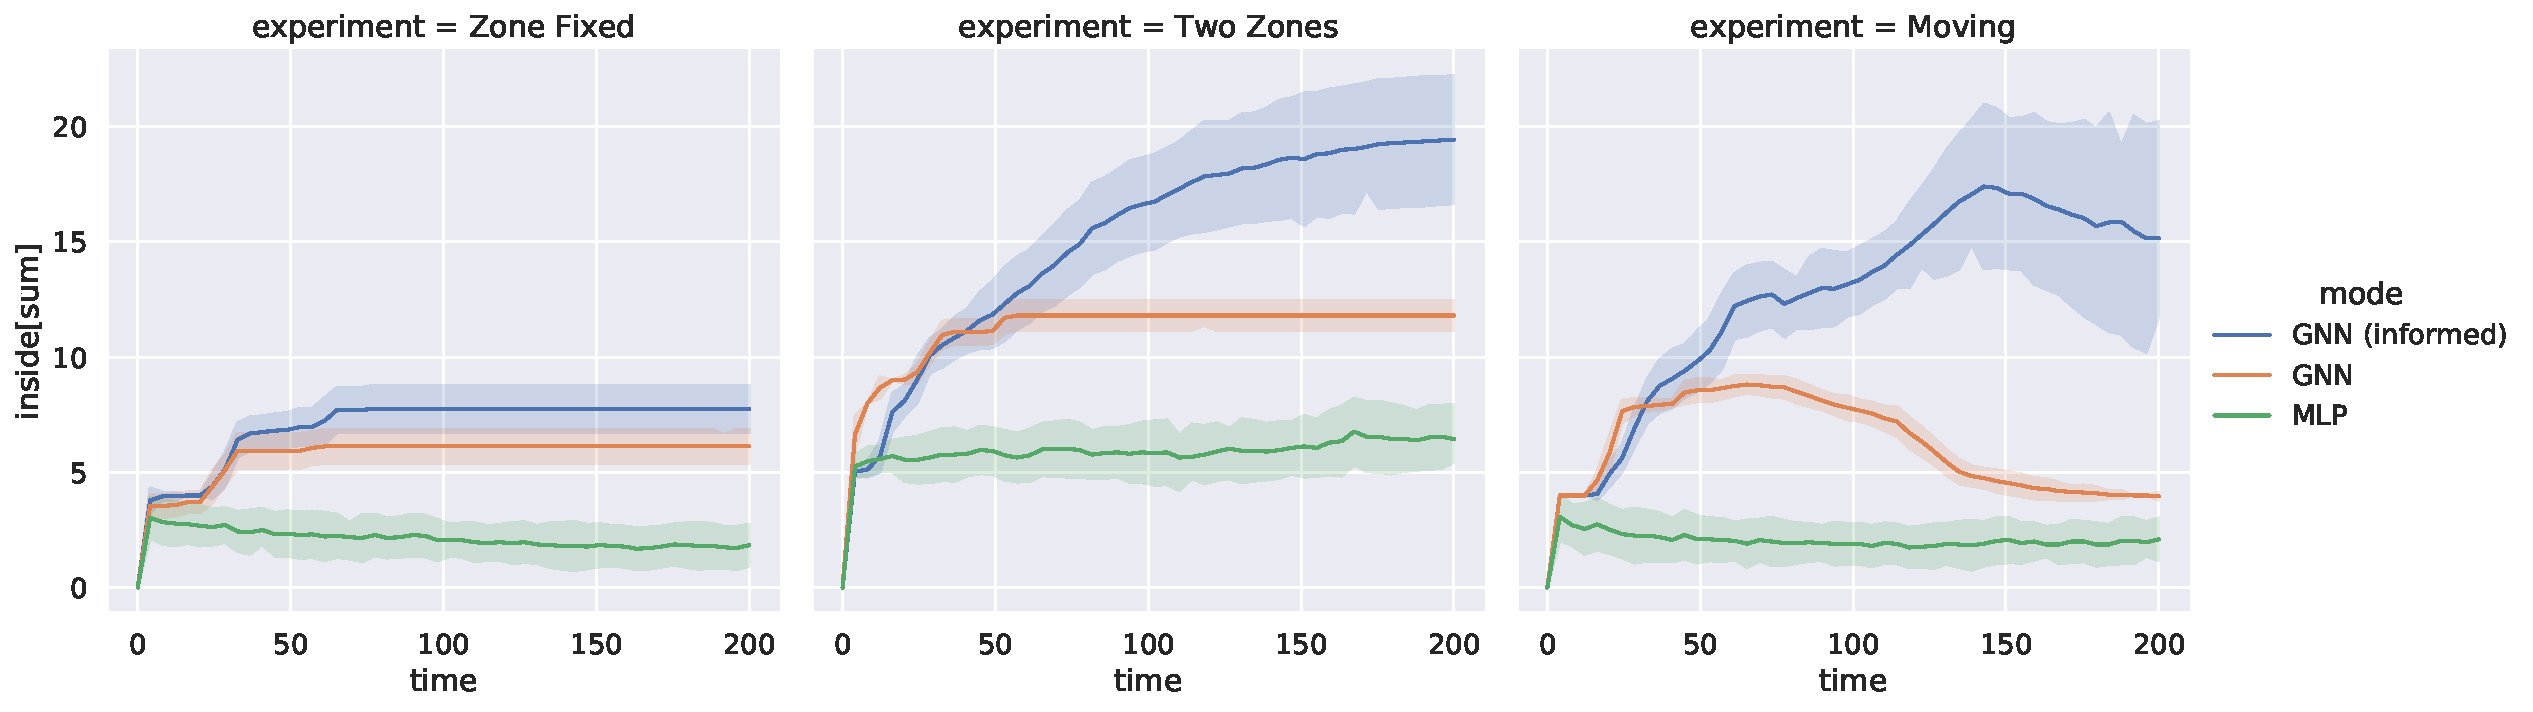
\includegraphics[width=\linewidth]{imgs/inside-test}
    \caption{Number of agents inside the phenomenon in the three types of experiments}
    \label{fig:inside-test}
  \end{subfigure}
	\caption{Quantative test results in the three types of scenarios.
	 	We can see that the proposed approach is able to cover and track the phenomenon better than the baselines.
	}
	\label{fig:test}
\end{figure*}

\begin{figure*}
	\centering
  	\begin{subfigure}[b]{0.85\linewidth}
    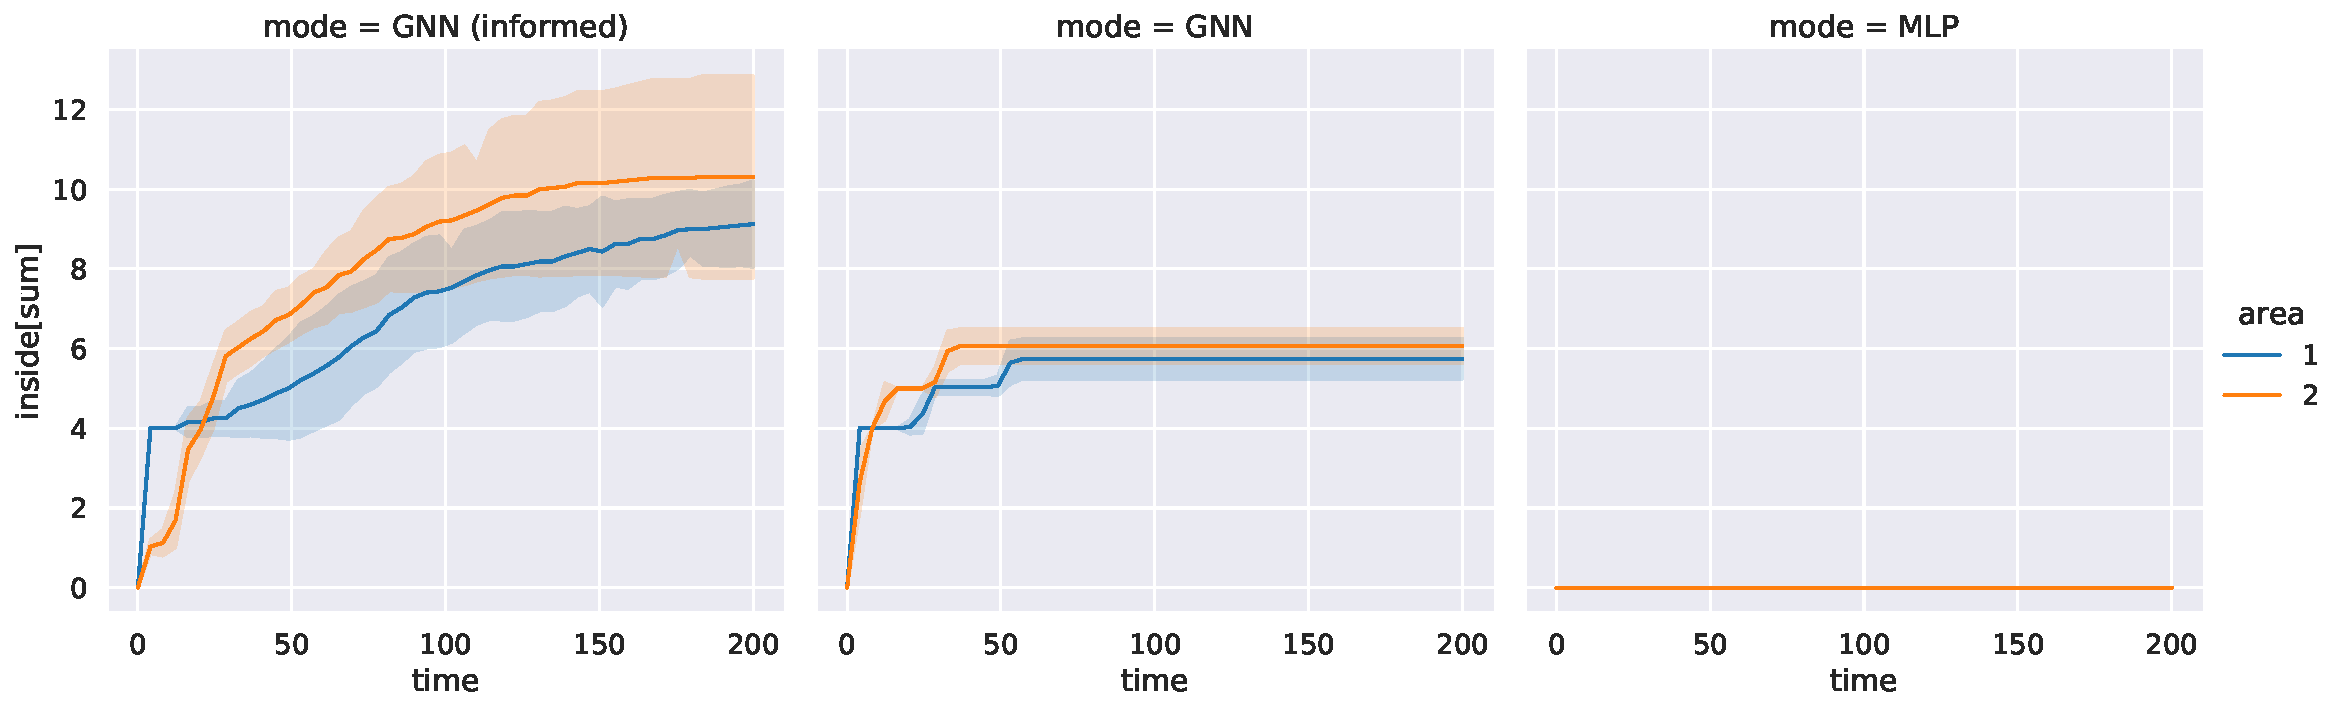
\includegraphics[width=\linewidth]{imgs/inside-two-test}
    \caption{\emph{Two Zones} experiment: aggregated number of agent inside each phenomenon}
    \label{fig:inside-two-test}
  \end{subfigure}
  \begin{subfigure}[b]{0.85\linewidth}
    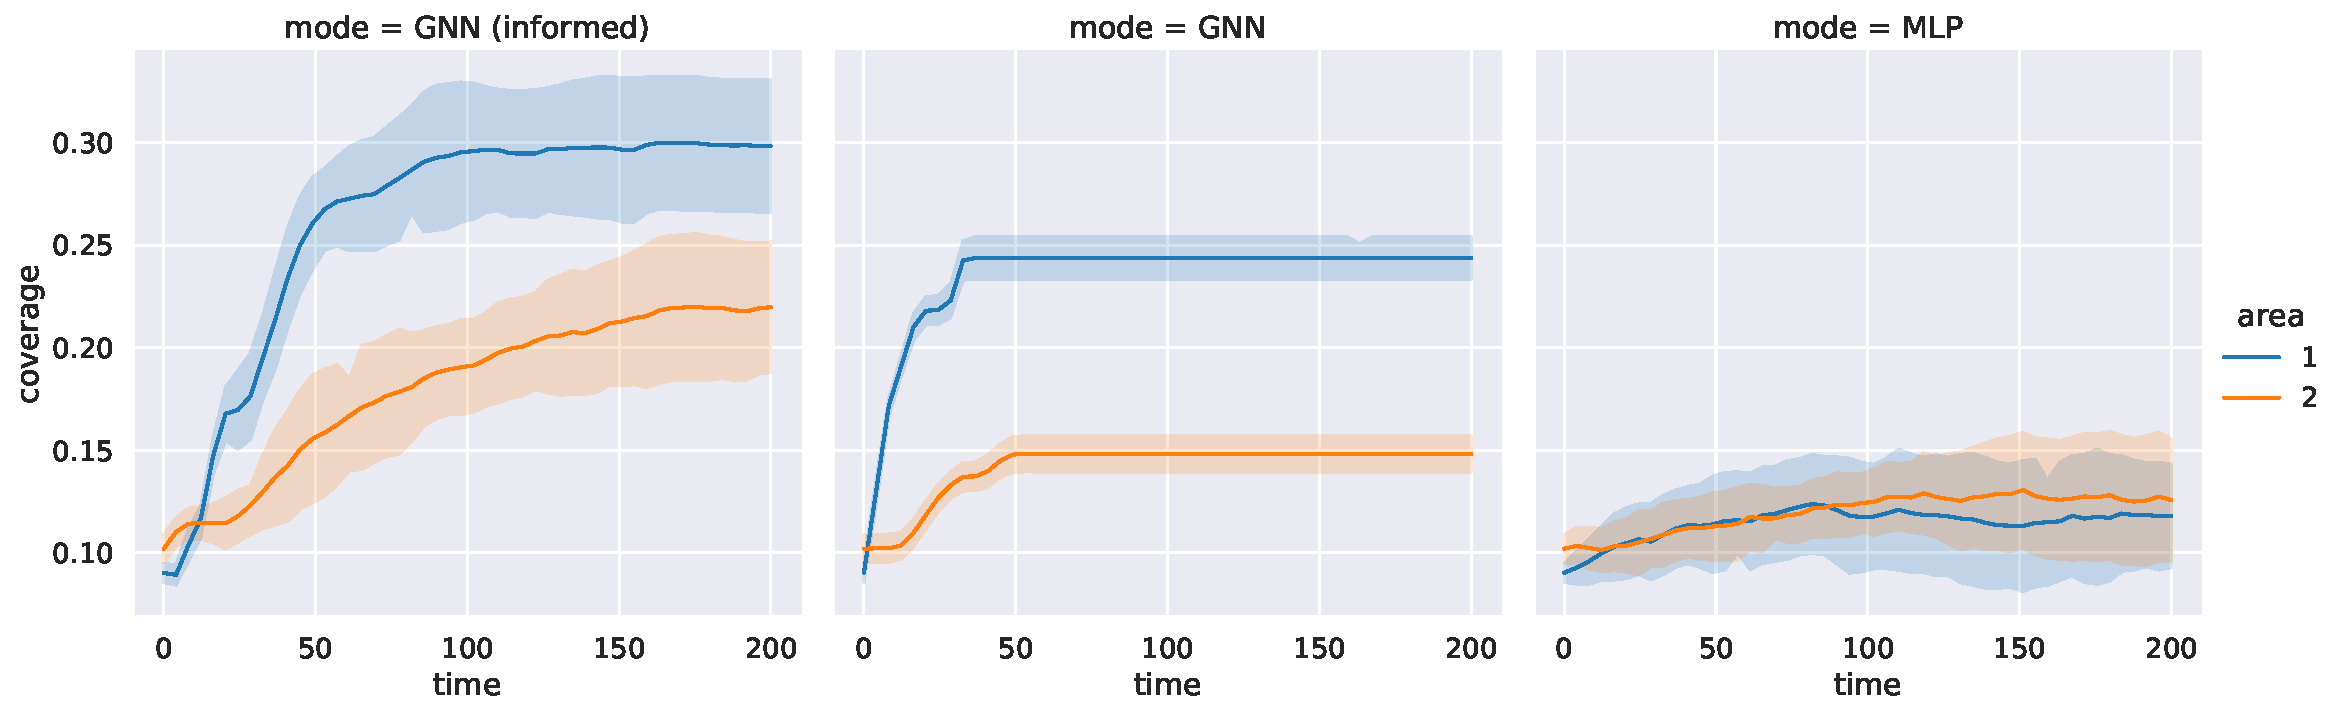
\includegraphics[width=\linewidth]{imgs/coverage-two-test}
    \caption{\emph{Two Zones} experiment: ratio of covered to the uncovered area both phenomena}
    \label{fig:coverage-two-test}
  \end{subfigure} 
  \caption{Coverage of two zones using the different modes of the controller.}
  \label{fig:resCoverage}
\end{figure*}
 
\section{Conclusion and Future Work}
In this paper, 
 we have introduced a novel approach for constructing distributed controllers by leveraging aggregate computing to encode agent interactions, 
 along with the combination of \ac{DQN} and \ac{GNN} for synthesizing distributed intelligence.
The proposed \emph{Field-Informed reinforcement learning} (FIRL) approach offers a promising solution to the challenges faced in coordinating multi-agent systems. 
By combining manual design and machine learning techniques, 
 the approach enables agents to autonomously learn and adapt their behaviour while leveraging locally available information. 
%
The demonstrated success in the proposed case study in solving collective tasks underscores the potential impact of this approach in advancing the field of multi-agent systems and swarm robotics. 

Future research could explore its application in diverse domains and evaluate its scalability and robustness in increasingly complex scenarios. 
%
In addition, we also plan to take the approach to modern actor-critical solutions, which are better suited to modern swarm robotics problems because of the continuous action space.
%\ga{Page budget: 0.5}
\label{sec:conclusion}

\bibliographystyle{IEEEtran}
\bibliography{bibliography}

\end{document}
